\chapter{Introduction}
\label{chap:intro}
\section{Hydrodynamic Stability and Parallel Shear Flows}
What is hydrodynamic stability? Hydrodynamic stability is the area of fluid mechanics associated with the stability of flows or systems of flow. For virtually any system where a fluid is in motion, hydrodynamic stability is something that must be considered. This includes obvious examples such as rivers or pipes, but also less obvious examples such as blood flowing through vessels.

We see an example of hydrodynamic stability almost every day when we go to turn on a tap. In some cases, the stream of water appears completely clear. This is an example of \emph{laminar flow} and is a visual example of a stable flow. In other cases, possibly even if we change how far we turn the handle / open the same tap (i.e. change the speed at which the water leaves the tap), the stream appears 'cloudy'. This is an example of unstable or \emph{turbulent flow} and appears when the velocity profile of the stream isn't stable. Different taps will display this behaviour at different points when they are turned. This is due to their nozzles having different shapes and also having water flowing through them at different speeds. This nicely demonstrates the impact that changing the velocity and also the channel shape of a flow can have on the stability of a flow. Figure \ref{fig:tapflow} shows an example of a tap producing a stable flow (left) versus an unstable flow (right).

\begin{figure}[h!]
    \centering
    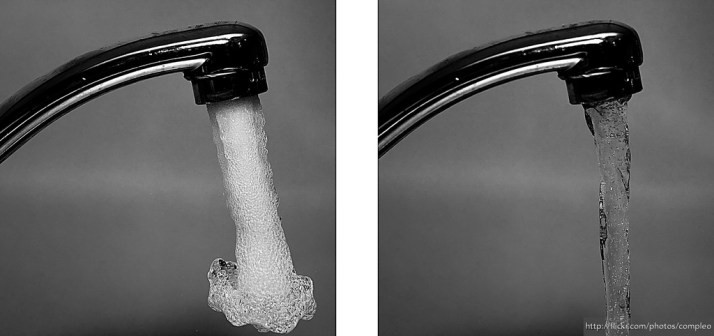
\includegraphics[width=13cm, keepaspectratio]{figures/StablevUnstable.jpg}
    \caption{Turbulent flow versus stable laminar flow from a tap (\href{https://www.flowvis.org/2018/01/30/7640/}{\textcolor{blue}{Image source})}}
    \label{fig:tapflow}
\end{figure}

Another property of a fluid that affects its stability is \emph{viscosity}. In the example of a tap, the most common fluid present is water which has a very low viscosity. However, if it was something like oil or syrup leaving the tap the viscosity is much higher. Figure \ref{fig:viscousflow} shows a number of fluids of increasing viscosity being poured from identical test tubes. How does this affect stability? From what we see in real life, we'd expect viscosity to have a stabilising effect since a fluid like vegetable oil or honey seems a lot more stable when poured than water. The fluids in Figure \ref{fig:viscousflow} seem to show this too, with the least viscous fluid on the left looking more unstable that the more viscous fluids on its right.

\begin{figure}[h!]
    \centering
    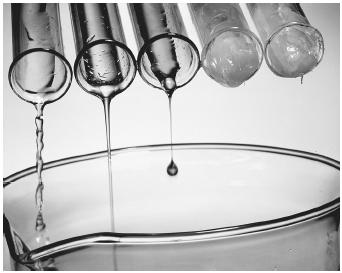
\includegraphics[width=80mm]{figures/viscosity-liquids.jpg}
    \caption{Fluids of increasing viscosity being poured from test tubes. The least viscous fluid is on the left and the most viscous fluid is on the right. (\href{https://schoolworkhelper.net/what-is-viscosity-application-flow-factors/}{\textcolor{blue}{Image source})}}
    \label{fig:viscousflow}
\end{figure}

A parallel shear flow is an axisymmetric flow with parallel streamlines. A plane flow is a 2-dimensional flow i.e. the flow is occurring only in one plane e.g. the $(x, z) $ plane. This report aims to determine the stability of 2-dimensional viscous parallel shear flows, otherwise known as viscous plane flows. 

The most common real-life example of this flow is that of a flow where a fluid is flowing through a pipe or other channel (such as a river bed). This is an important concern in the real world, due to the fact that energy equivalent to roughly 10\% of the world's electricity is used moving fluids through pipes. A significant source of additional cost is turbulence since it involves the fluid swirling around itself and therefore not taking the most efficient path through the pipe. Figure \ref{fig:pipeflow} shows a comparison between turbulent flow (top) and stable flow (bottom) in a pipe. 

\begin{figure}[h!]
    \centering
    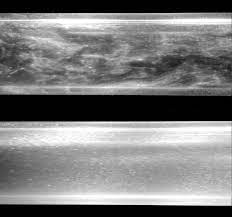
\includegraphics[width=80mm]{figures/pipe_turb.jpg}
    \caption{Turbulent pipe flow (top) versus stable pipe flow (bottom) - (\href{https://www.pumpindustry.com.au/research-reveals-better-manage-turbulence-in-pipes/}{\textcolor{blue}{Image source})}}
    \label{fig:pipeflow}
\end{figure}

In the inviscid case, there are many known analytic results on the stability of parallel shear flows such as \emph{Rayleigh's inflexion point theorem} \citep{rayleigh1880stability} which states that a necessary condition for instability is that the velocity profile contains an inflexion point. 

However, in the viscous case, the analytic results are far less concrete. Some do exist, such as the bounds found by \citet{synge1938hydrodynamical, pai1954generalization} and \cite{joseph1968eigenvalue, joseph1969eigenvalue}, but as will be shown, they are extremely approximate, and do not tell us much about the stability of a specific flow. For this reason, numerical methods are often used instead. The aim of this report is to demonstrate both these analytic results on stability and a numerical method that can be used to more accurately determine the stability of the flow. 

\section{Outline of this report}
Chapter \ref{chap:governing} will introduce the basic state and governing equations for viscous plane flows, along with the family of flows that we are studying, plane Poiseuille and plane Couette flow. The chapter will then turn to manipulating these governing equations, reducing them to just a single equation, the Orr-Sommerfeld equation. The Orr-Sommerfeld equation is an extremely significant equation when studying the linear stability of viscous parallel shear flows, and will be the equation that this report will use to provide both numerical and analytical results on stability.

Chapter \ref{chap:suffcons} contains a discussion on how the Orr-Sommerfeld equation derived in Chapter \ref{chap:governing} can be used to determine whether a flow is stable or not, before deriving separate equations for both the real and imaginary parts of the eigenvalue. We then turn to derive bounds on the real part of the eigenvalue, otherwise known as the wave speed. We derive bounds as seen in \citet{pai1954generalization, joseph1968eigenvalue} which restrict the eigenvalues to a strip in the complex plane. We then derive bounds on the imaginary part of the eigenvalue, deriving the bounds found by \citet{synge1938hydrodynamical, joseph1968eigenvalue, joseph1969eigenvalue}. This gives us two bounds on the stability of a flow and allows us to get an analytic estimate of the critical Reynolds number of Couette and Poiseuille flow. However, these are extremely inaccurate, causing us to seek out a numerical method.

Chapter \ref{chap:numerics} turns to a numerical method to determine the stability of a flow. The numerical methods in question involve the use of Chebyshev polynomials and are referred to as the Chebyshev Tau methods. In the Chebyshev Tau method, we expand our function in terms of Chebyshev polynomials and represent the coefficients of this expansion in a vector. To represent the derivatives we use a matrix that transforms the coefficients of our expansion vector. This produces a matrix system that allows us to determine whether a flow is stable based on its eigenvalues. In the Tau method, the eigenvectors are the coefficients of the Chebyshev polynomial expansion representing our eigenfunctions. This chapter features 3 different ways of forming the generalised eigenvalue problem that we solve in Python, each using a larger system of lower-order differential equations. The reason we perform this split is to reduce the numerical error associated with the extremely large values present in the matrices we are using. This chapter will also explain which eigenvalue algorithm will be used to solve the generalised eigenvalue problems generated by each of our problems.

The numerical results of these methods are discussed in Chapter \ref{chap:results}, followed by a comparison and discussion of the methods used and their advantages and disadvantages. The first set of results shown will be for the case of plane Poiseuille flow, but the chapter will then turn to discuss the results for the case of plane Couette flow. This chapter then turns to show several other key numerical results that we can get from our programs, such as the eigenfunctions (and associated streamfunctions) and the critical Reynolds number. 

